\documentclass[a4paper,12pt]{article}
\usepackage[utf8]{inputenc}
\usepackage{geometry} % to change the page dimensions
\geometry{margin=2.5cm} % set up margins 
\usepackage{graphicx} % to include \includegraphics command and options
\usepackage[parfill]{parskip} % Activate to begin paragraphs with an empty line rather than an indent
\usepackage{authblk}
%\usepackage{kpfonts} % kind of font
\usepackage[colorlinks=true]{hyperref}
\usepackage[portuguese]{babel}
\usepackage{fancybox, graphicx}
\usepackage{microtype}

\title{Tutorial de instalação Anaconda/Python/Jupyter}
\author{Prof. Gustavo Oliveira, gustavo.oliveira@ci.ufpb.br}
\affil{Departamento de Computação Científica, CI/UFPB}
\date{}

\begin{document}
\maketitle


\abstract{Tutorial básico de instalação de ferramentas suficientes para a execução de \emph{Jupyter notebooks} em \texttt{Python 3.x}}

\subparagraph{\scriptsize{Última atualização: \today.}}

\section{Apresentação}

Este tutorial foi desenvolvido para dar suporte aos estudantes do curso
de Cálculo Numérico da Universidade Federal da Paraíba nas turmas ministradas pelo
autor. Seu objetivo específico é ensinar o procedimento de instalação de
ferramentas computacionais básicas para a execução dos arquivos
\emph{Jupyter notebook} (formato \texttt{.ipynb}) pertencentes ao
programa suplementar de aprendizado de computação numérica desenvolvido
para a disciplina.

\section*{Por que Anaconda?}

A instalação de um interpretador Python é uma tarefa simples. No
entanto, a instalação dos pacotes adicionais necessários para as tarefas
de computação numérica apresentadas no curso, tais como as bibliotecas
NumPy, SciPy, Sympy e Matplotlib, pode tornar-se um pouco mais
trabalhosa. Por esta razão, optamos pela distribuição Anaconda, a qual,
além de fornecer o interpretador Python e todos esses pacotes, também
permite a execução simples e direta da interface Jupyter. A distribuição
Anaconda (\url{https://www.continuum.io/what-is-anaconda}) é multiplataforma, 
ou seja, está disponível para os sistemas Windows, Linux e macOS, e de uso gratuito.

\section*{Por que Jupyter?}

O Projeto Jupyter (\url{http://jupyter.org}) é um projeto de código aberto nascido do Projeto
IPython em 2014, voltado para o suporte à ciência de dados interativa e
computação científica em todas as linguagens de programação. O Jupyter é
um software de código 100\% aberto e gratuito para uso pela comunidade
global e lançado sob os termos da licença BSD modificada.

\section*{Que versão Python usar?}

Existem duas versões de Python usuais: Python 2.x e Python 3.x. Elas são
levemente diferentes. As mudanças na Python 3.x foram introduzidas para
corrigir algumas deficiências no projeto da linguagem identificados
desde o seu início. Uma decisão que foi tomada assumiu que alguma
incompatibilidade deveria ser aceita para se atingir o objetivo maior de
uma linguagem melhor para o futuro. Em virtude de a tendência ser sempre
de melhorias, usaremos a versão Python 3.x

\section*{Como instalar a distribuição Anaconda?}

\begin{enumerate}
\item
  Acesse o link \url{https://www.continuum.io/downloads} e faça o
  download do software para seu sistema operacional. Role a página para
  baixo até a respectiva aba de seu sistema operacional. Opte pela
  versão Python 3.6 (atual). Uma tela aparecerá onde você poderá
  preencher o seu e-mail e fazer o download de uma folha de dicas (cheat
  sheet), se desejar. Caso contrário, clique em \texttt{NO,\ THANKS}
  para que o processo de download
  comece.\footnote{O tamanho do arquivo de instalação pode variar de sistema para sistema.}
\item
  Execute o arquivo de instalação que você acabou de baixar para seu
  computador e siga os passos de instalação normalmente.
\end{enumerate}

\section*{Como lançar o Jupyter Notebook?}

\begin{enumerate}
\item
  Abra o \emph{Anaconda Navigator}. O ícone se parece com a figura \ref{fig:icon}:
\begin{figure}[h!]
\centering
\caption{\label{fig:icon}Ícone do Anaconda.}
\shadowbox{
\includegraphics[scale=1.5]{figs/icon.png}}
\end{figure}  
\item
  No \emph{Anaconda Navigator}, clique no botão \texttt{Home} no menu
  lateral à direita para acessar a janela inicial (caso não seja aberta
  automaticamente). Vide figura \ref{fig:home}.
\begin{figure}[h!]
\centering
\caption{\label{fig:home}Janela inicial do \emph{Anaconda Navigator}.}
\shadowbox{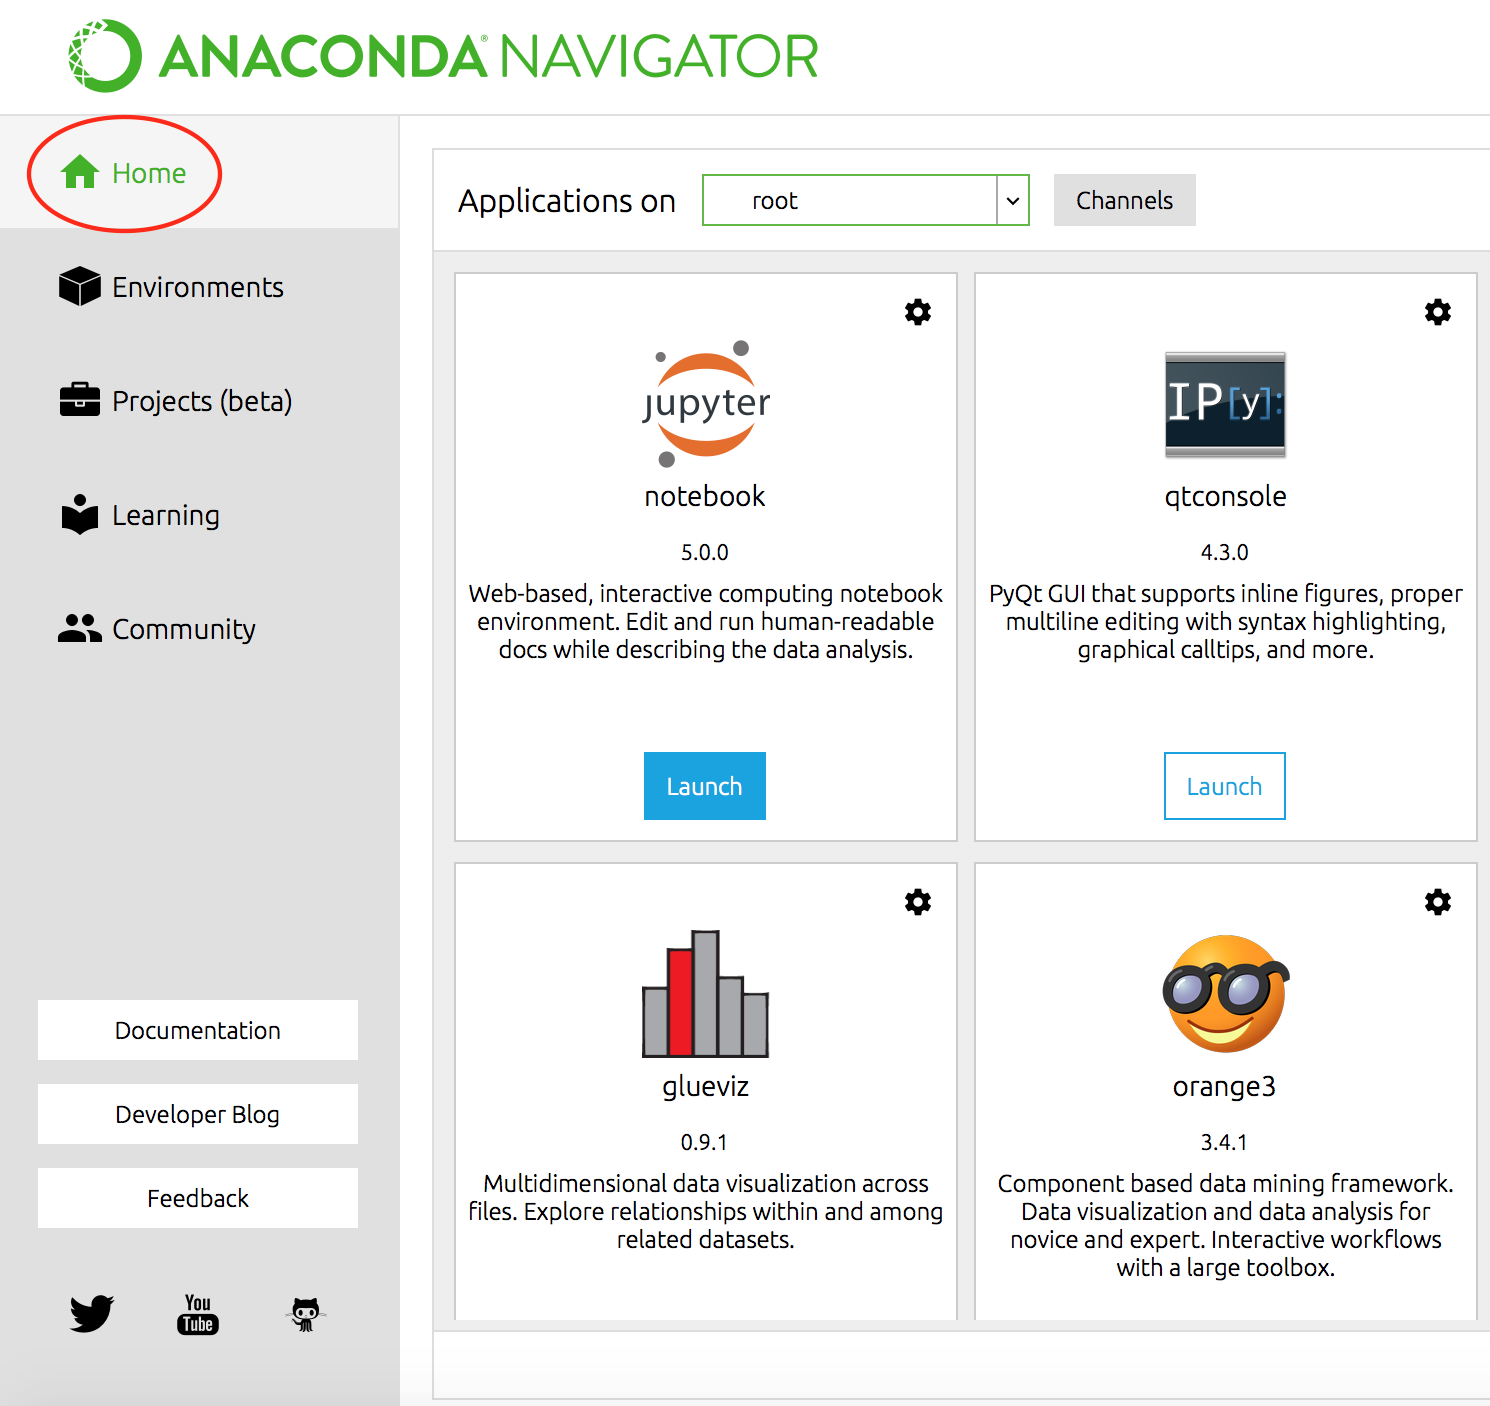
\includegraphics[scale=0.5]{figs/home.png}}
\end{figure}  
\item
  Abra o \emph{Jupyter Notebook} clicando no respectivo botão
  \texttt{Launch}. Vide figura \ref{fig:launch}.
  \begin{figure}[h!]
\centering
\caption{\label{fig:launch}Botão de lançamento do Jupyter.}
\shadowbox{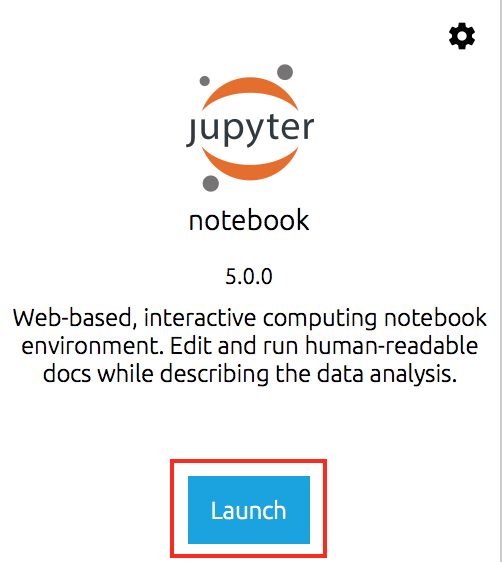
\includegraphics[scale=0.5]{figs/launch.png}}
\end{figure}  
\item
  Em seguida, uma aba deverá abrir em seu navegador padrão com a tela
  inicial do Jupyter mostrando o seu diretório de
  usuário.\footnote{Se alguma tela mencionando algum erro de execução aparecer ao tentar lançar o Jupyter, tente abri-lo digitando o endereço \url{http://localhost:8890} diretamente na barra de endereço de uma nova aba que você deve abrir em seu navegador. Isto quer dizer que o Jupyter está rodando em um servidor local, seu computador.}
\item
  Navegue pelos diretórios até à pasta onde você salvou os arquivos
  \texttt{.ipynb}. Neste exemplo, eles estão no caminho
  \texttt{courses/calculo-numerico/lecture-ipynb}. Vide figura \ref{fig:jupyter}.
\begin{figure}[h!]
\centering
\caption{\label{fig:jupyter}Tela inicial do \emph{Jupyter} aberta em uma nova janela ou aba de seu navegador.}
\shadowbox{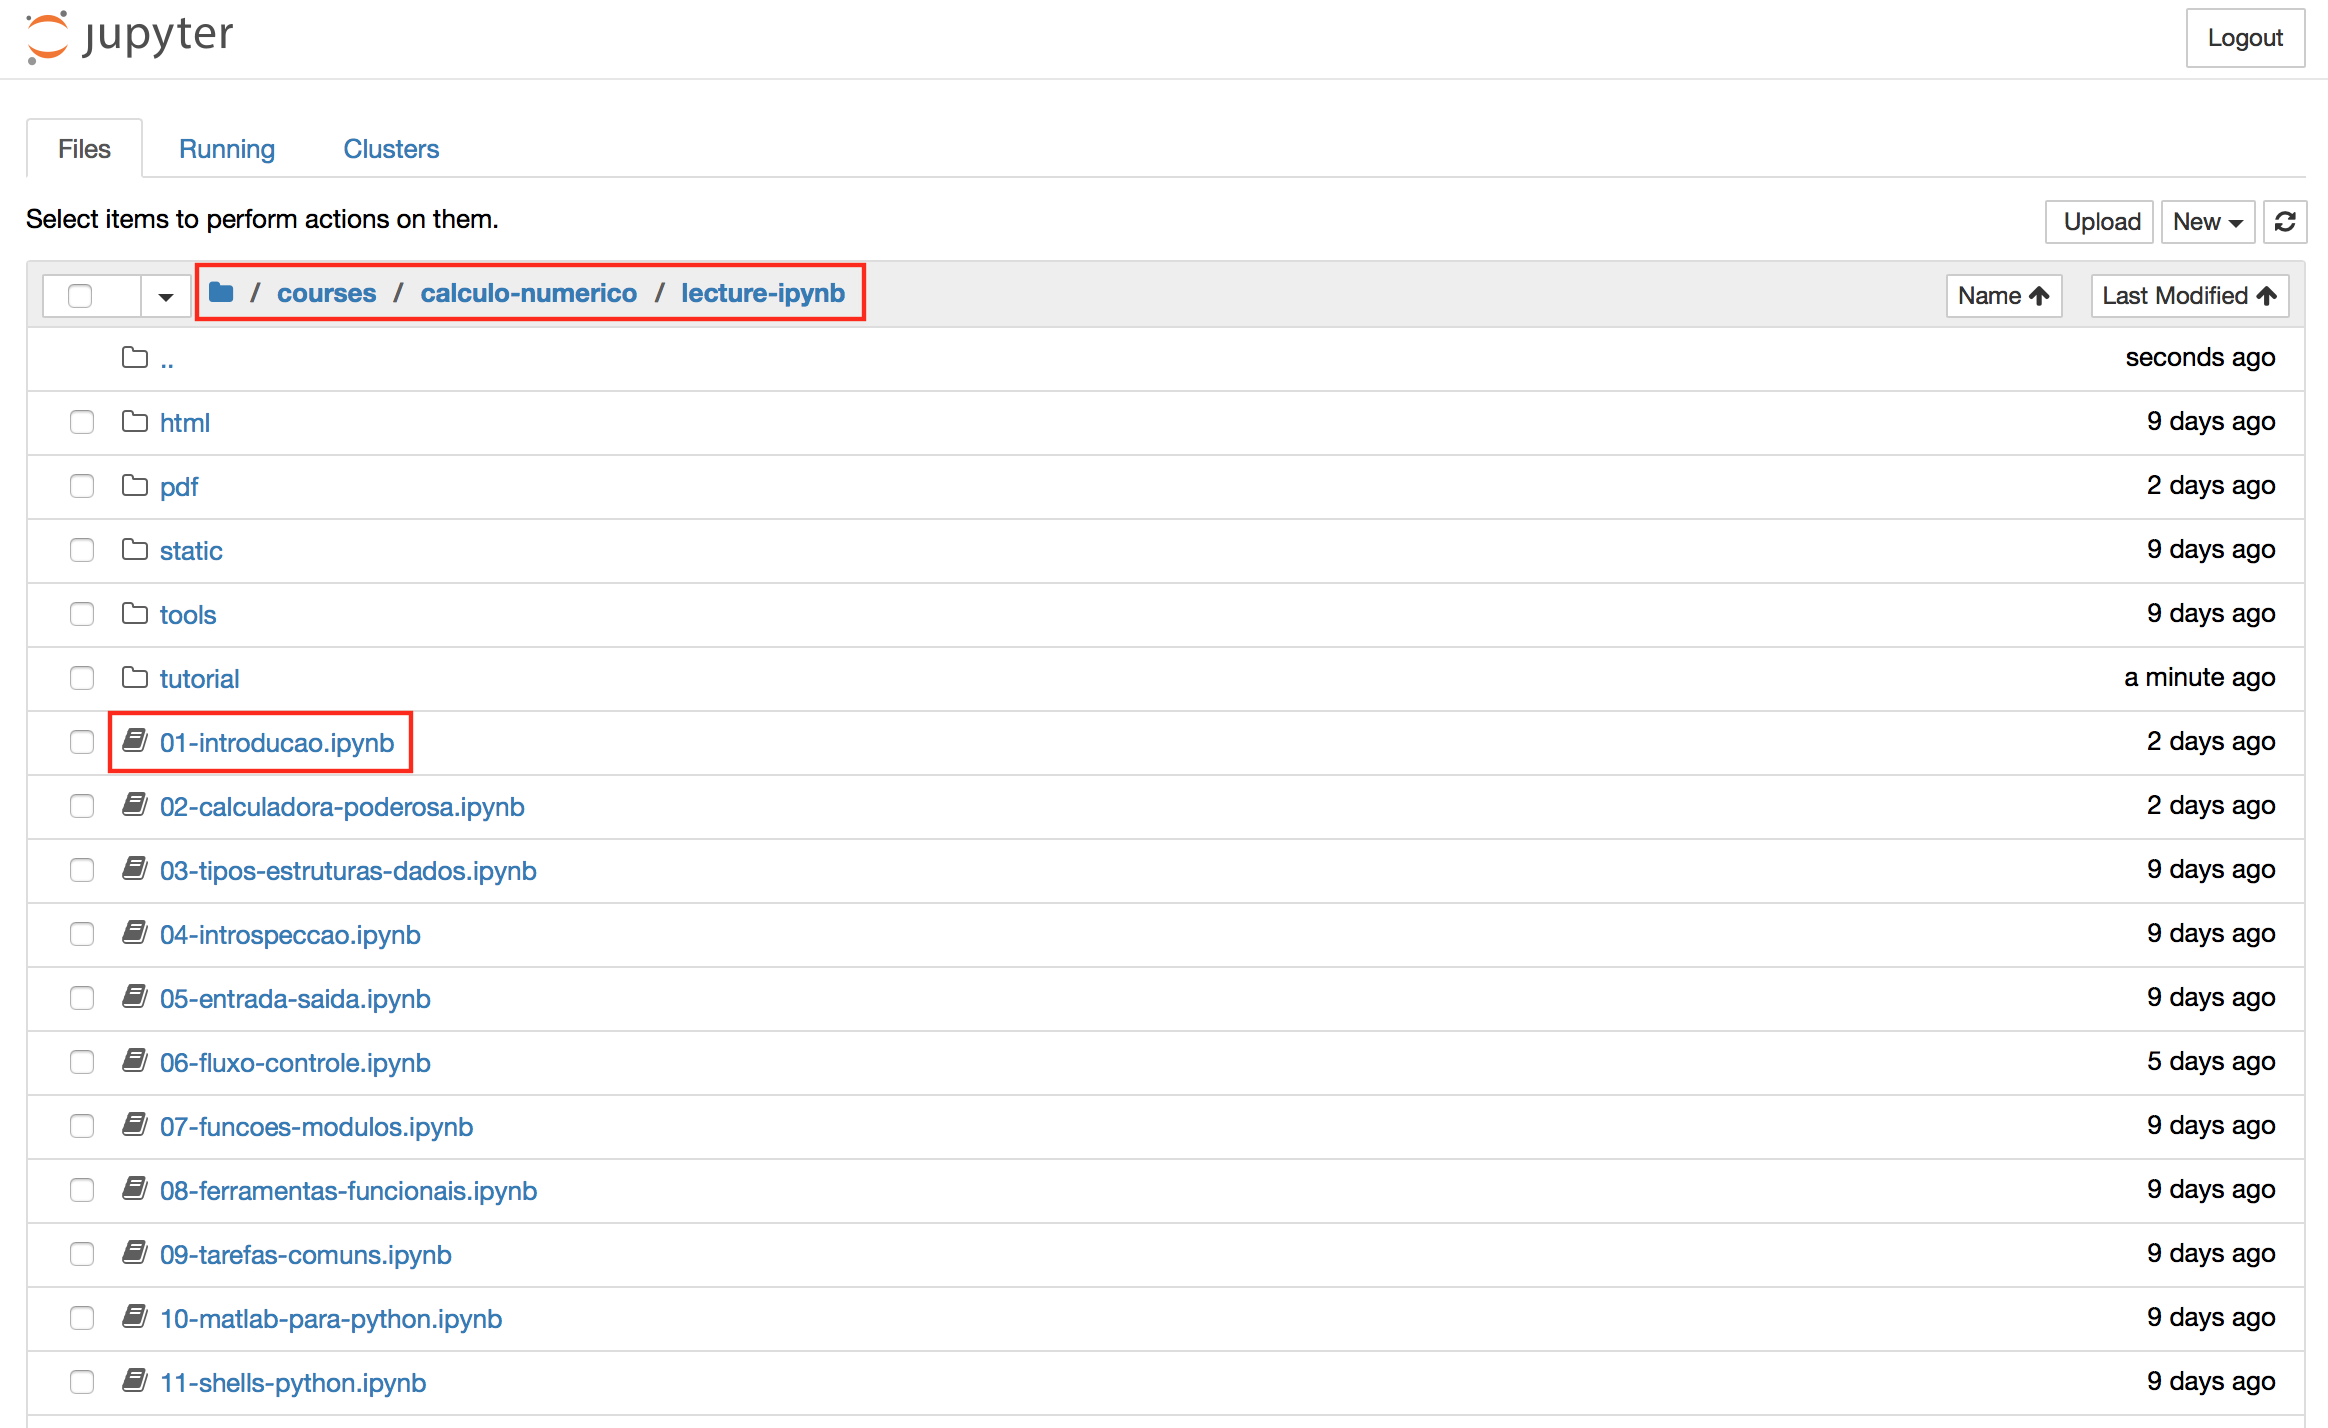
\includegraphics[scale=0.4]{figs/jupyter.png}}
\end{figure}  
\item
  Abra os arquivos \texttt{.ipynb} clicando em seus nomes. Uma tela como
  a da figura a seguir deve ser lançada quando clicarmos no arquivo
  \texttt{01-introducao.ipynb}, por exemplo. Observe que um indicador da versão \texttt{Python 3} aparece no canto superior direito da tela. Vide figura \ref{fig:intro}. Todos os demais arquivos podem ser abertos da mesma maneira. 
  \begin{figure}[h!]
\centering
\caption{\label{fig:intro}Tela inicial do \emph{Jupyter} aberta em uma nova janela ou aba de seu navegador.}
\shadowbox{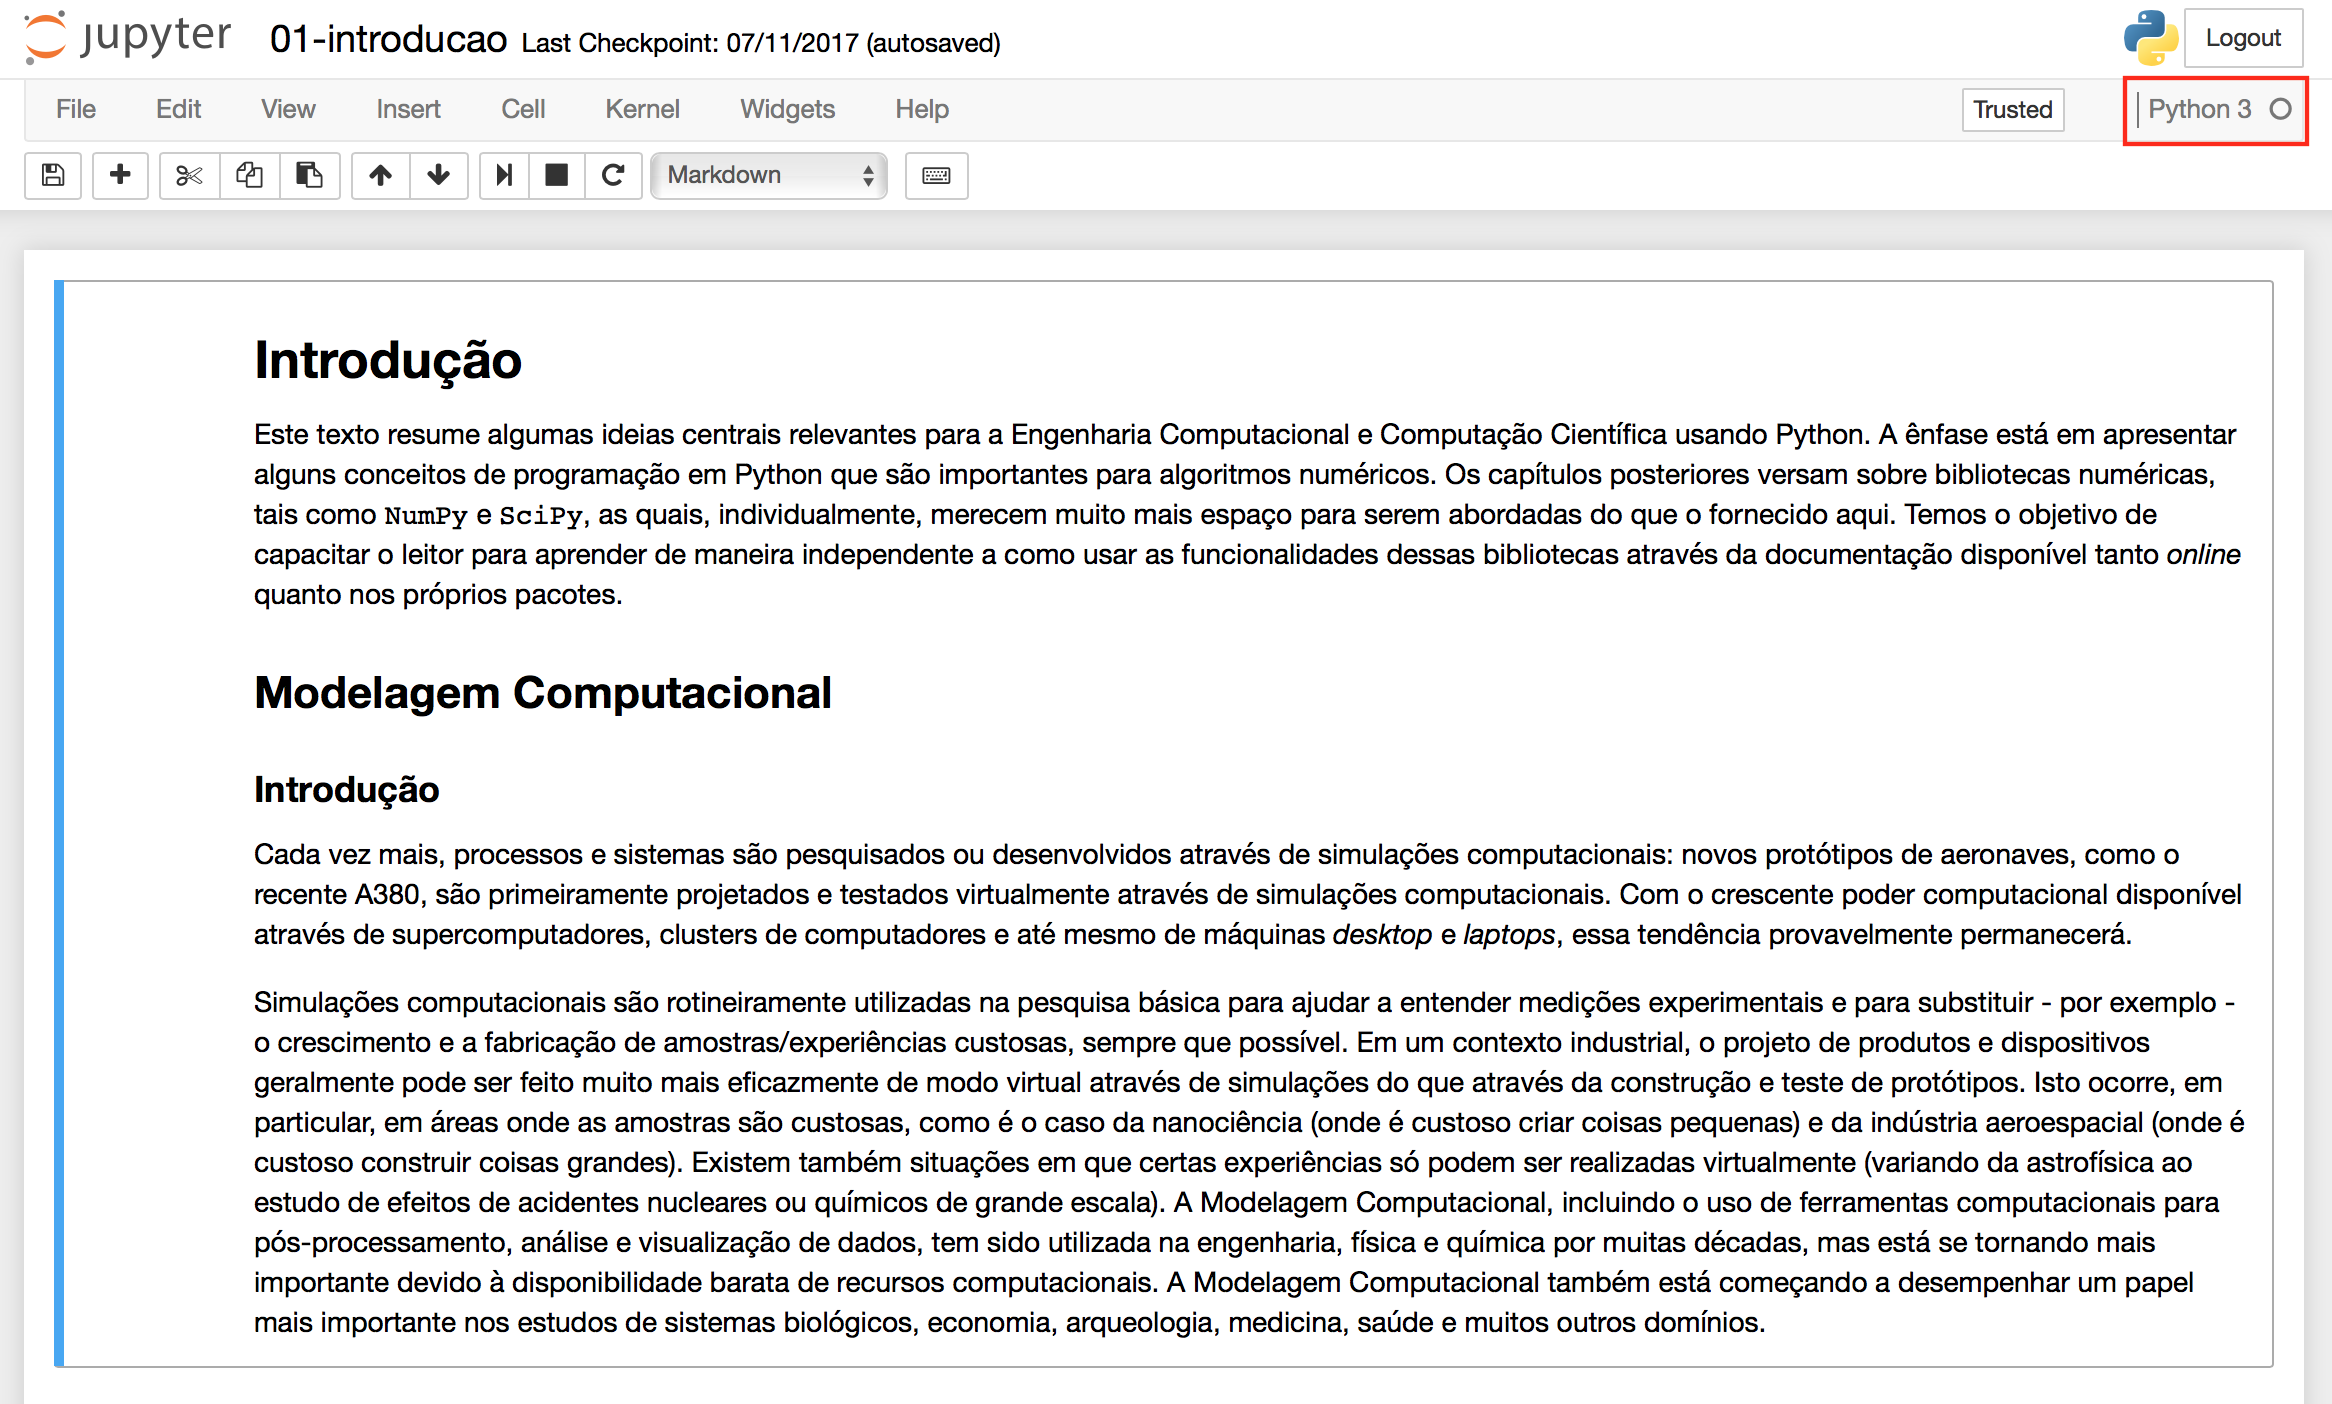
\includegraphics[scale=0.4]{figs/intro.png}}
\end{figure}  
\end{enumerate}

\section*{Como encerrar a execução?}

Depois de terminar de usar o seu arquivo \texttt{.ipynb}, feche a aba ou janela onde ele está sendo executado, vá até a aba onde você o lançou, selecione o arquivo e clique em \texttt{Shutdown}. Em seguida, feche as janelas que estiverem abertas por ocasião do \emph{Anaconda Navigator}. Vide \ref{fig:shutdown}.
 \begin{figure}[h!]
\centering
\caption{\label{fig:shutdown}Tela inicial do Jupyter destacando o encerramento da execução atual.}
\shadowbox{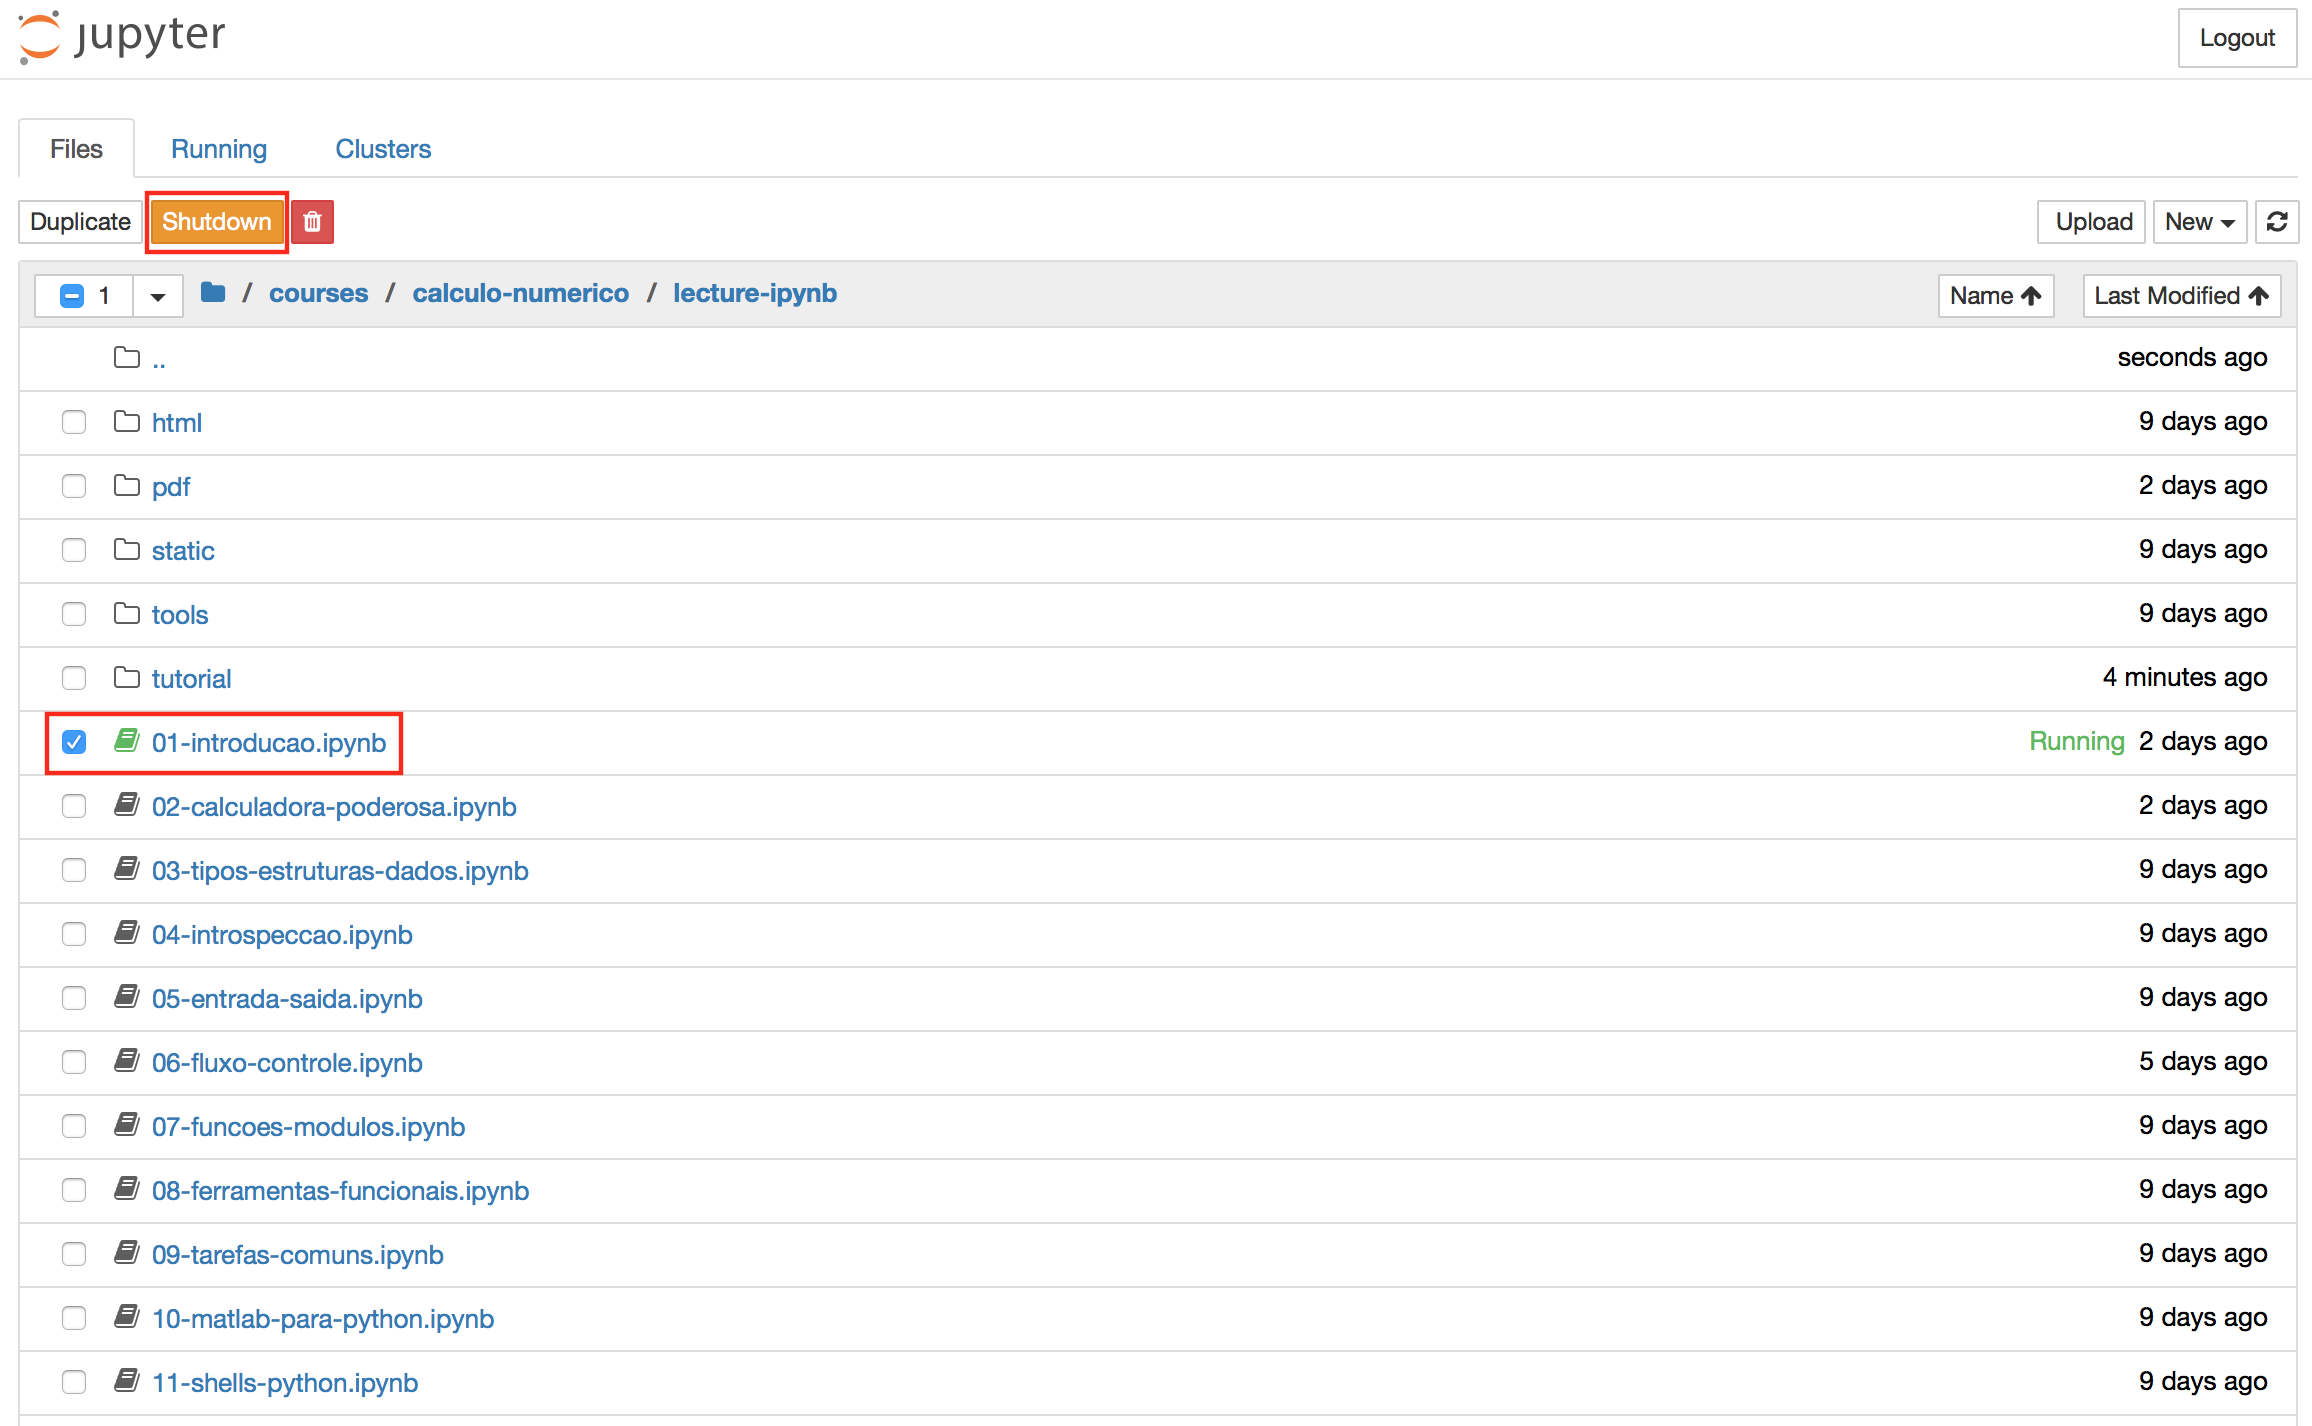
\includegraphics[scale=0.4]{figs/shutdown.png}}
\end{figure}  

\section*{Sugestões, correções e comentários}

Todos são bem-vindos! Caso tenha comentários ou sugestões a fazer, ou se encontrou algum erro e deseje apontar correções, não hesite em contatar o autor. Este material será revisto e atualizado frequentemente, podendo ser expandido conforme necessidade. 

\end{document}
